
\subsection{Análisis Paramétrico de la Modulación FSK en Tiempo y Frecuencia}
Se analizó el comportamiento de la señal modulada FSK ante variaciones de la frecuencia portadora ($f_c$) y la desviación de frecuencia ($f_d$). En el dominio del tiempo, como se observa en la Figura \ref{fig:fsk_tiempo}, se comprobó que un incremento en $f_c$ resulta en una compresión del periodo de la señal de RF, aumentando la densidad de las oscilaciones por símbolo, mientras que la tasa de baudios permanece constante.

\begin{figure}[H]
    \centering
    \subfloat[Baja frecuencia portadora ($f_c = 12$ kHz).]{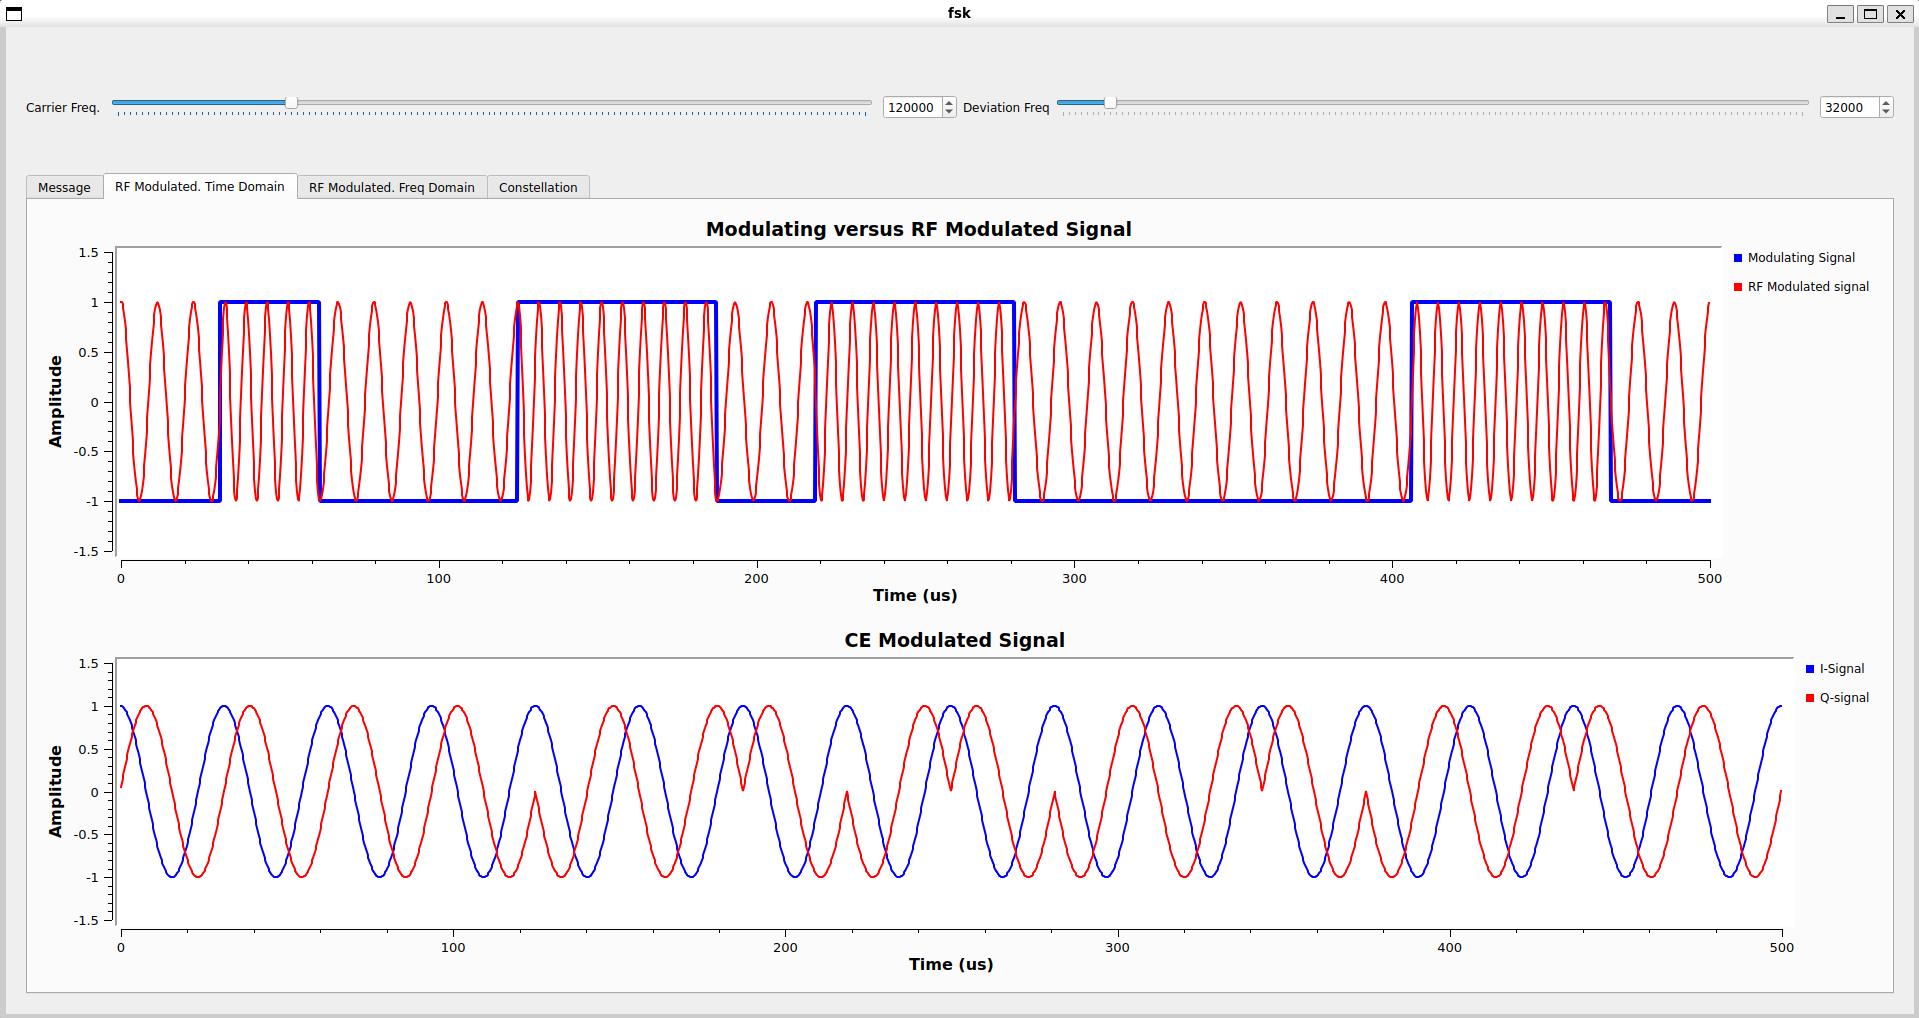
\includegraphics[width=0.48\linewidth]{imagenes/señal_modulada_punto_8_fc_12000_df_32000.png}\label{fig:t1}}
    \hfill
    \subfloat[Alta frecuencia portadora ($f_c = 30$ kHz).]{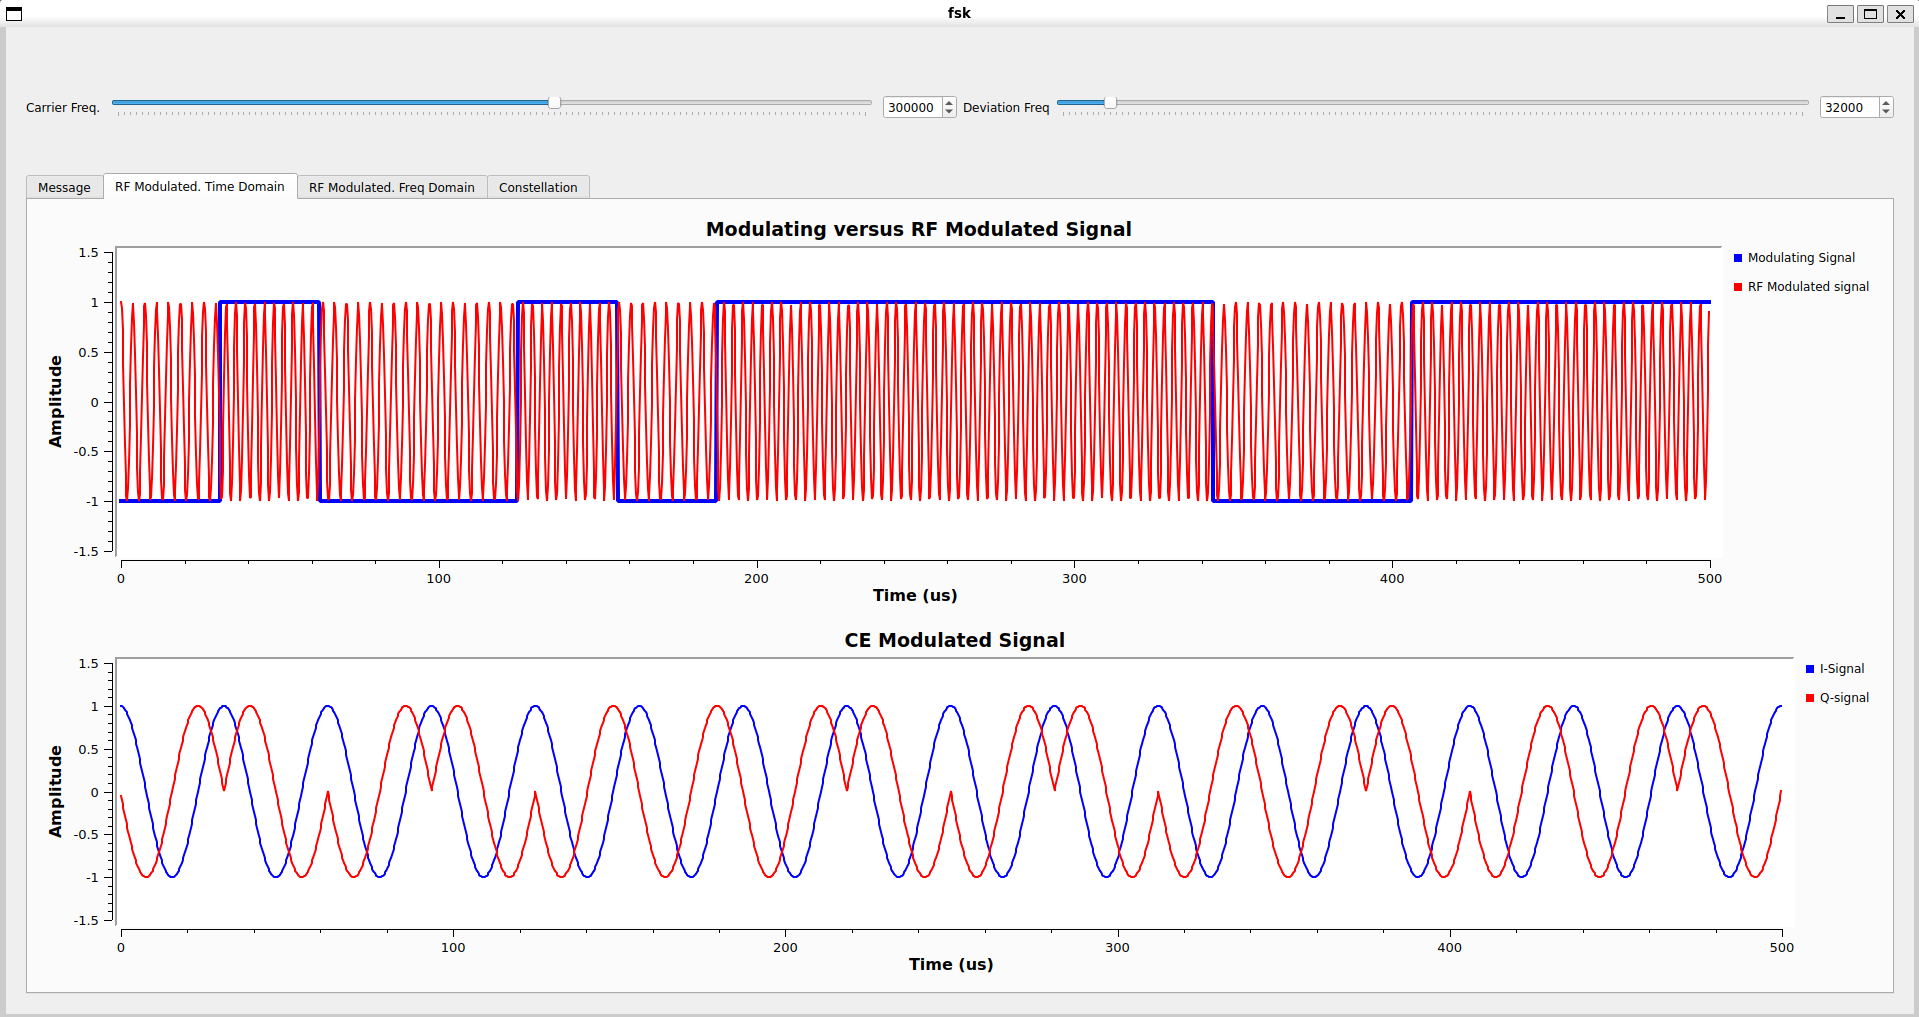
\includegraphics[width=0.48\linewidth]{imagenes/señal_modulada_punto_8_fc_30000_df_32000.png}\label{fig:t2}}
    \caption{Representación temporal de la señal FSK para diferentes valores de portadora.}
    \label{fig:fsk_tiempo}
\end{figure}

En el dominio de la frecuencia, se identificó que la Envolvente Compleja (EC) presenta una inmunidad total ante cambios en la portadora, manteniéndose centrada en 0 Hz independientemente del valor de $f_c$. No obstante, la desviación $f_d$ demostró ser el parámetro determinante del ancho de banda y la integridad espectral en ambos dominios (RF y EC). 

Como se evidencia en la Figura \ref{fig:fsk_frec}, una desviación reducida ($f_d = 2$ kHz) provoca un solapamiento severo entre los tonos ortogonales, dificultando la recuperación de la información. Por el contrario, una configuración de $f_d = 32$ kHz proporciona una separación clara de los lóbulos en RF ($f_c \pm f_d$) y en EC ($\pm f_d$), minimizando la interferencia.

\begin{figure}[H]
    \centering
    \subfloat[Solapamiento espectral crítico ($f_d = 2$ kHz).]{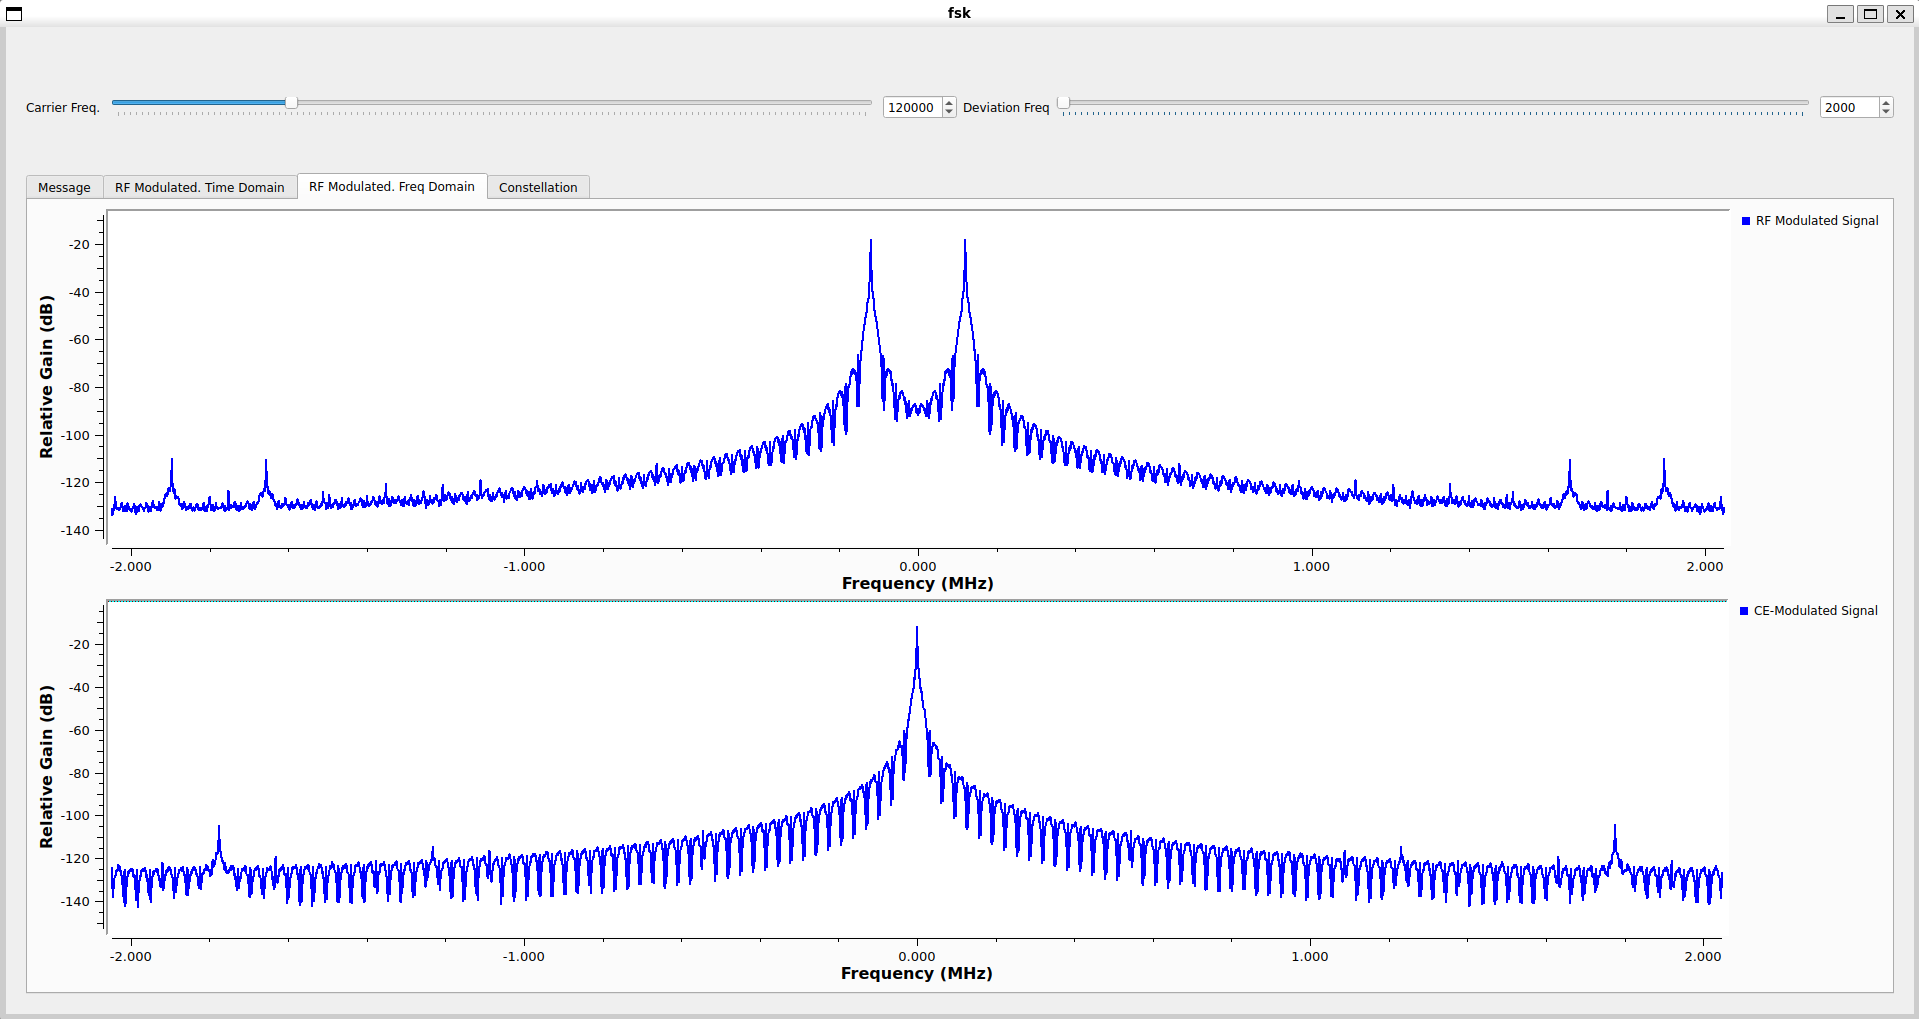
\includegraphics[width=0.48\linewidth]{imagenes/dominio_en_frecuencia_fc_120000_df_2000_punto_8.png}\label{fig:f1}}
    \hfill
    \subfloat[Separación espectral adecuada ($f_d = 32$ kHz).]{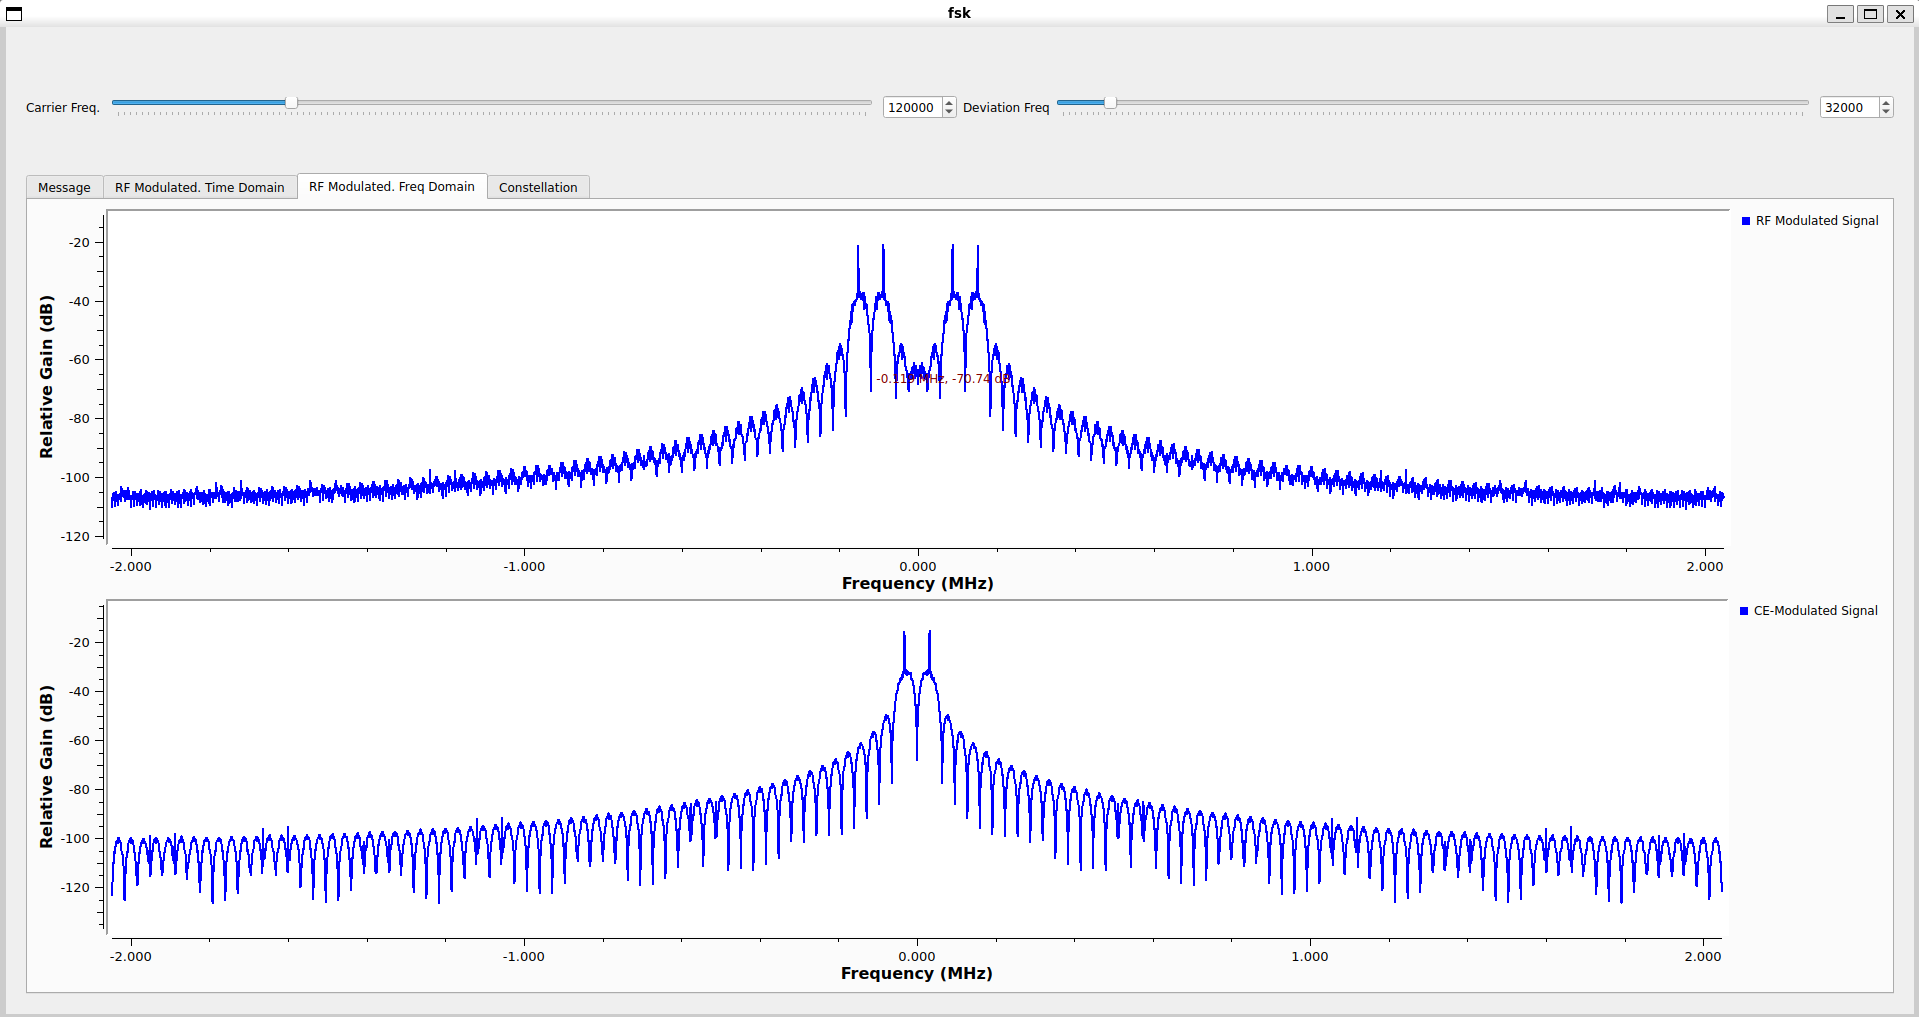
\includegraphics[width=0.48\linewidth]{imagenes/dominio_en_frecuencia_fc_120000_df_32000_punto_8.png}\label{fig:f2}}
    \caption{Densidad espectral de potencia (PSD) variando la desviación de frecuencia.}
    \label{fig:fsk_frec}
\end{figure}

Para sintetizar el comportamiento observado, la Tabla \ref{tab:resumen_fsk} resume la dependencia de los dominios de simulación frente a los parámetros de control. Se concluye que mientras $f_c$ actúa como un factor de traslación frecuencial puro para la componente de RF, $f_d$ gobierna la dinámica interna de la fase, afectando la ocupación espectral de forma global.

\begin{table}[h]
\centering
\caption{Sensibilidad Paramétrica de la Simulación FSK}
\label{tab:resumen_fsk}
\begin{tabular}{|l|c|c|c|}
\hline
\textbf{Parámetro} & \textbf{Dominio Tiempo} & \textbf{Espectro RF} & \textbf{Espectro EC} \\ \hline
Variación $f_c$ & Modifica periodo & Traslación & Inmune \\ \hline
Variación $f_d$ & Modifica fase & Ancho banda & Ancho banda \\ \hline
\end{tabular}
\end{table}